\documentclass{article}
\usepackage{graphicx}
\usepackage{wrapfig}
\usepackage{filecontents}
\usepackage{siunitx}
\usepackage[table]{xcolor}
\usepackage{float}
\usepackage{hyperref}

\usepackage{color} % balíček pro obarvování textů
\usepackage{xcolor}  % zapne možnost používání barev, mj. pro \definecolor
\usepackage{pgfplots} % http://www.chiark.greenend.org.uk/doc/texlive-doc/latex/pgfplots/pgfplots.pdf

\ifnum 0\ifxetex 1\fi\ifluatex 1\fi=0 % if pdftex
  \usepackage[T1]{fontenc}
  \usepackage[utf8]{inputenc}
\else % if luatex or xelatex
  \ifxetex
    \usepackage{mathspec}
  \else
    \usepackage{fontspec}
  \fi
  \defaultfontfeatures{Ligatures=TeX,Scale=MatchLowercase}
\fi
\usepackage[total={175mm,230mm}, top=23mm, left=20mm, includefoot]{geometry}
\hypersetup{
    colorlinks,
    linkcolor={blue!50!black},
    citecolor={green!50!black},
    urlcolor={blue!80!black}
}
\definecolor{orange}{RGB}{ 251, 114, 032}
\definecolor{fialova}{RGB}{ 255, 000, 255}

\newcommand \obr[1]
{ obr.~\ref{#1}}

\newcommand \tab[1]
{ tab.~ß\ref{#1}}


\begin{document}
\pagestyle{empty}

\definecolor{color_29791}{rgb}{0,0,0}
\begin{figure}[H]
    \hspace{-13mm}
    \begin{minipage}[t]{\textwidth}
        \vspace{-20mm}
        \begin{tikzpicture}[overlay]
            \path(0pt,0pt);
        \end{tikzpicture}
        \begin{picture}(-5,0)(2.5,0)
            \put(123.656,-82.75397){\fontsize{18}{1}\usefont{T1}{ptm}{m}{n}\selectfont\color{color_29791}VYSOKÉ UČENÍ TECHNICKÉ V BRNĚ}
            \put(76.296,-104.785){\fontsize{13}{1}\usefont{T1}{ptm}{m}{n}\selectfont\color{color_29791}FAKULTA  ELEKTROTECHNIKY A KOMUNIKAČNÍCH TECHNOLOGIÍ}
            \put(198.447,-128.5339){\fontsize{16}{1}\usefont{T1}{cmr}{b}{n}\selectfont\color{color_29791}Ústav elektrotechnologie}
            \put(156.848,-278.1589){\fontsize{14}{1}\usefont{T1}{ptm}{m}{n}\selectfont\color{color_29791}LABORATORNÍ CVIČENÍ Z PŘEDMĚTU}
            \put(83.123,-300.2579){\fontsize{14}{1}\usefont{T1}{cmr}{b}{n}\selectfont\color{color_29791}ELEKTROTECHNICKÉ MATERIÁLY A VÝROBNÍ PROCESY}
            \put(55.85,-421.25){\fontsize{14}{1}\usefont{T1}{cmr}{b}{n}\selectfont\color{color_29791}Číslo úlohy: 6}
            \put(55.85,-469.547){\fontsize{14}{1}\usefont{T1}{cmr}{b}{n}\selectfont\color{color_29791}Název úlohy: Počítačové vytváření pásových modelů polovodičových materiálů}
            \put(23.9,-620.32){\fontsize{12}{1}\usefont{T1}{cmr}{b}{n}\selectfont\color{color_29791}Jméno a příjmení, ID:}
            \put(23.9,-637.119){\fontsize{12}{1}\usefont{T1}{cmr}{b}{n}\selectfont\color{color_29791}Tomáš Vavrinec, 240893}
            \put(186.95,-620.32){\fontsize{12}{1}\usefont{T1}{cmr}{b}{n}\selectfont\color{color_29791}Atmosférický tlak:}
            \put(186.95,-637.119){\fontsize{12}{1}\usefont{T1}{cmr}{b}{n}\selectfont\color{color_29791}102.6 hPa}
            \put(293.25,-620.32){\fontsize{12}{1}\usefont{T1}{cmr}{b}{n}\selectfont\color{color_29791}Teplota okolí: }
            \put(293.25,-637.119){\fontsize{12}{1}\usefont{T1}{cmr}{b}{n}\selectfont\color{color_29791}25.1°C}
            \put(417.25,-620.32){\fontsize{12}{1}\usefont{T1}{cmr}{b}{n}\selectfont\color{color_29791}Relativní vlhkost:}
            \put(417.25,-637.119){\fontsize{12}{1}\usefont{T1}{cmr}{b}{n}\selectfont\color{color_29791}37.2\%}
            \put(23.9,-665.77){\fontsize{12}{1}\usefont{T1}{cmr}{b}{n}\selectfont\color{color_29791}Měřeno dne:}
            \put(23.9,-682.569){\fontsize{12}{1}\usefont{T1}{cmr}{b}{n}\selectfont\color{color_29791}14.10.2022}
            \put(186.95,-665.77){\fontsize{12}{1}\usefont{T1}{cmr}{b}{n}\selectfont\color{color_29791}Odevzdáno dne:}
            \put(293.25,-665.77){\fontsize{12}{1}\usefont{T1}{cmr}{b}{n}\selectfont\color{color_29791}Ročník, stud. skupina:}
            \put(293.25,-682.569){\fontsize{12}{1}\usefont{T1}{cmr}{b}{n}\selectfont\color{color_29791}2}
            \put(417.25,-665.77){\fontsize{12}{1}\usefont{T1}{cmr}{b}{n}\selectfont\color{color_29791}Kontrola:}
            \put(23.9,-703.42){\fontsize{12}{1}\usefont{T1}{cmr}{b}{n}\selectfont\color{color_29791}Spolupracovali:}
            \put(23.9,-720.219){\fontsize{12}{1}\usefont{T1}{cmr}{b}{n}\selectfont\color{color_29791}Daniel Poisl}
        \end{picture}
        \begin{tikzpicture}[overlay]
            \path(0pt,0pt);
            \draw[color_29791,line width=0.5pt]
            (20.4pt, -606.117pt) -- (20.4pt, -722.815pt)
            ;
            \draw[color_29791,line width=0.5pt]
            (183.45pt, -606.117pt) -- (183.45pt, -651.067pt)
            ;
            \draw[color_29791,line width=0.5pt]
            (183.45pt, -651.567pt) -- (183.45pt, -688.717pt)
            ;
            \draw[color_29791,line width=0.5pt]
            (289.75pt, -606.117pt) -- (289.75pt, -651.067pt)
            ;
            \draw[color_29791,line width=0.5pt]
            (289.75pt, -651.567pt) -- (289.75pt, -688.717pt)
            ;
            \draw[color_29791,line width=0.5pt]
            (413.75pt, -606.117pt) -- (413.75pt, -651.067pt)
            ;
            \draw[color_29791,line width=0.5pt]
            (413.75pt, -651.567pt) -- (413.75pt, -688.717pt)
            ;
            \draw[color_29791,line width=0.5pt]
            (544.9pt, -606.117pt) -- (544.9pt, -722.815pt)
            ;
            \draw[color_29791,line width=0.5pt]
            (20.15pt, -605.867pt) -- (545.15pt, -605.867pt)
            ;
            \draw[color_29791,line width=0.5pt]
            (20.65pt, -651.317pt) -- (544.65pt, -651.317pt)
            ;
            \draw[color_29791,line width=0.5pt]
            (20.65pt, -688.967pt) -- (544.65pt, -688.967pt)
            ;
            \draw[color_29791,line width=0.5pt]
            (20.15pt, -723.065pt) -- (545.15pt, -723.065pt)
            ;
            \draw[color_29791,line width=1.5pt]
            (15.75pt, -15.59998pt) -- (15.75pt, -729pt)
            ;
            \draw[color_29791,line width=1.5pt]
            (549.55pt, -15.59998pt) -- (549.55pt, -729pt)
            ;
            \draw[color_29791,line width=1.5pt]
            (15.75pt, -729pt) -- (549.55pt, -729pt)
            ;
            \draw[color_29791,line width=1.5pt]
            (15pt, -14.84998pt) -- (550.3pt, -14.84998pt)
            ;
        \end{tikzpicture}
    \end{minipage}
\end{figure}

\newpage
\pagestyle{plain}


\subsection*{Zadání}
Určete driftovou pohyblivost minoritních nosičů a sledujte její změnu s měnící se intenzitou elektrického pole.
Graficky znázorněte závislost pohyblivosti minoritních nosičů proudu na intenzitě elektrického pole.
\begin{figure}[H]
    \hspace{0.05\textwidth}
    \begin{minipage}[t]{0.9\textwidth}
        \begin{figure}[H]
            \begin{minipage}[t]{0.6\textwidth}
                Na emitor přiložte impulsy\\
                Stejnosměrný proud vzorkem nastavujte v rozmezí\\
                Změřte vzdálenost hrotů (d)\\
            \end{minipage}
            \hfill
            \begin{minipage}[t]{0.4\textwidth}
                \(t = (5 - 20) [\mu s] \)\\
                \(I = (5 - 35) [mA] \) min. 10 hodnot\\
            \end{minipage}
        \end{figure}
    \end{minipage}
    
    \hspace{0.05\textwidth}
    \begin{minipage}[t]{0.9\textwidth}
        \begin{figure}[H]
            \begin{minipage}[t]{0.6\textwidth}
                \textbf{ Parametry vzorku a použitých materiálů}\\
                Rezistivita vzorku křemíku je \\
                Průřez vzorku je\\
                Vzdálenost hrotů je nutné změřit\\
            \end{minipage}
            \hfill
            \begin{minipage}[t]{0.4\textwidth}
                \vspace{1.5mm}
                \(\rho = 0.464\-[\mu m]\)\\
                \(S = (1.5 x 5)\-[mm^2]\)\\
            \end{minipage}
        \end{figure}
    \end{minipage}
\end{figure}

\subsection*{Teoretický úvod}
Normálně se v krystalu pohybují nosiče náboje nahodile všemi směry, dohromady se tedy proud který tvoří vykompenzuje.
Po vložení krystalu do elektrického pole \(E\) se k náhodnému pohyby přičte pohyb v opačném směru než ve kterém působí el.pole.
Rychlost tohoto pohybu značíme \(V_{drift}\) a definujeme vztahem \(V{drift} = E\cdot \mu_{drift}\) kde \(\mu_{drift}\) je driftová pohyblivost.
Vzhledem k tomu, že předpokládáme dva druhy nosičů, elektrony a díry, uvažujeme i jejich různé pohyblivosti.

Pokud do krystalu, kterým protéká proud (je tedy trvale el.poli) vyšleme pomocí dvou elektrod ojedinělý impulz, můžeme na druhé straně pozorovat tento impulz "rozdvojený".
Hlavní část impulzu je přenesena majoritními nosiči a sekundární pulz, který následuje těsně za hlavním je tvořen nosiči minoritními.
Ze vzdálenosti těchto dvou pulzů můžeme určit pohyblivost minoritních nosičů podle vztahu \(\mu = \frac{d}{E\cdot t_0}\) kde \(d\) je vzdálenost mezi elektrodami, \(E\) je intenzita el.pole a \(t_0\) je doba mezi impulzu.

Intenzitu el.pole můžeme spočítat podle vztahu \(E = \frac{U}{d} = \frac{\rho I}{S}\)

\begin{figure}[H]
    \centering
    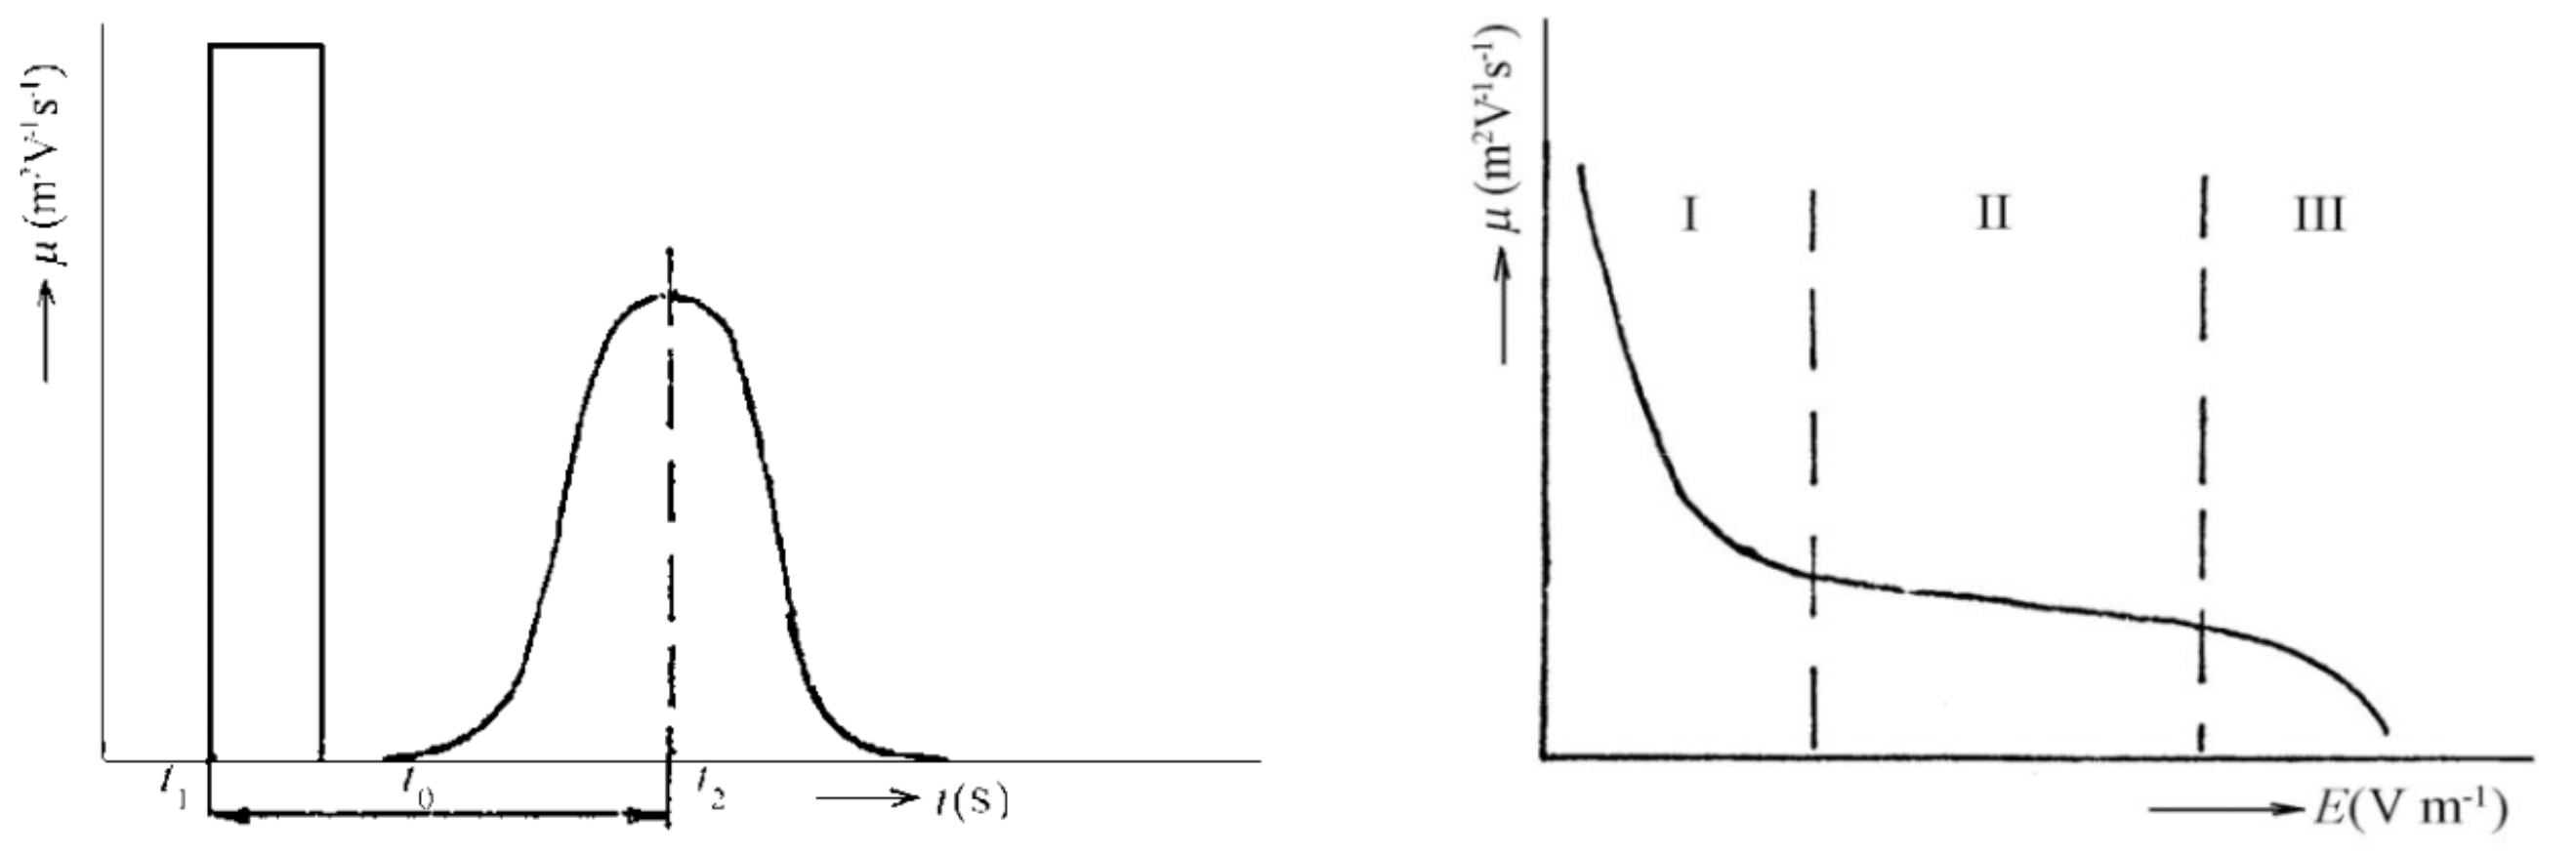
\includegraphics[width=0.7\textwidth]{pulzi_a_pad.png}
\end{figure}

\newpage
\hspace{-8mm}
\begin{tabular}{ccc}
    vzdálenost hrotů \(d = 1.8\-[mm]\) & měrná vodivost vzorku \(\rho = 0.464\-[\Omega m]\) & plochá průřezu vzorku \(S = 7.5\cdot10^{-6}\-[m^2]\) \\
\end{tabular}
\vspace{-5mm}
\begin{figure}[H]
    \begin{minipage}[t]{0.5\textwidth}
        \vspace{-100mm}
        \hspace{0.1\textwidth}
        \begin{table}[H]
            \centering
            \caption{\label{tabulka_mereni} Naměřené a vypočtené hodnoty}
            \begin{tabular}{|c|c|c|c|}
                \hline
                \(t0 [\mu s]\)	& \(I [mA]\)	& \(E [V/m]\)   & \(\mu [m^2V^{-1}s^{-1}]\) \\ \hline
                14.62	        &  5	        &  309.3        & 0.398                     \\ \hline
                14.68	        &  8	        &  494.9        & 0.248                     \\ \hline
                15.00	        & 10	        &  618.7        & 0.194                     \\ \hline
                15.08	        & 12	        &  742.4        & 0.161                     \\ \hline
                15.24	        & 14	        &  866.1        & 0.136                     \\ \hline
                15.44	        & 16	        &  989.9        & 0.118                     \\ \hline
                15.64	        & 18	        & 1113.6        & 0.103                     \\ \hline
                15.82	        & 20	        & 1237.3        & 0.092                     \\ \hline
                15.92	        & 22	        & 1361.1        & 0.083                     \\ \hline
                16.12	        & 24	        & 1484.8        & 0.075                     \\ \hline
                16.32	        & 26	        & 1608.5        & 0.069                     \\ \hline
                16.44	        & 28	        & 1732.3        & 0.063                     \\ \hline
                16.50	        & 30	        & 1856.0        & 0.059                     \\ \hline
                16.52	        & 32	        & 1979.7        & 0.055                     \\ \hline
                16.85	        & 34	        & 2103.4        & 0.051                     \\ \hline
            \end{tabular}
        \end{table}
        % \vspace{5mm}
        Příklad výpočtu el.pole \(E\) a pohyblivosti \(\mu \):\\
        \\
        \(
            E = \frac{\rho I}{S} = \frac{0.464\cdot5\cdot10^{-3}}{7.5\cdot10^{-6}} = 309.3\-[V/m]
        \)
        \\\\
        \(
            \mu = \frac{d}{E\cdot t_0} = \frac{1.8\cdot10^{-3}}{309.3\cdot14.62\cdot10^{-6}} = 0.398\-[m^2V^{-1}s^{-1}]
        \)\\
    \end{minipage}
    \hfill
    \begin{minipage}[t]{0.6\textwidth}
        \hspace{-0.1\textwidth}
        \begin{tikzpicture}
            \begin{axis}[
                    width=1\textwidth, 
                    height=100mm,
                    title={ závislost pohyblivosti \(\mu\) na intenzitě el.pole \(E\)},
                    xlabel={\(E\-[Vm^{-1}]\)},
                    ylabel={\(\mu\-[m^2V^{-1}s^{-1}]\)},
                    xmin=300, xmax=2200,
                    ymin=0.025, ymax=0.4,
                    xtick={0, 250, 500,..., 2000},
                    legend pos=north east,
                ]
                \addplot[
                  color=red,
                  mark=x,
                  ]
                  coordinates {
                    ( 309.3	 , 0.398)
                    ( 494.9	 , 0.248)
                    ( 618.7	 , 0.194)
                    ( 742.4	 , 0.161)
                    ( 866.1	 , 0.136)
                    ( 989.9	 , 0.118)
                    (1113.6	 , 0.103)
                    (1237.3	 , 0.092)
                    (1361.1	 , 0.083)
                    (1484.8	 , 0.075)
                    (1608.5	 , 0.069)
                    (1732.3	 , 0.063)
                    (1856.0	 , 0.059)
                    (1979.7	 , 0.055)
                    (2103.4	 , 0.051)
                };
                \addlegendentry{\scriptsize \(\mu_{mer}\)}
                \addplot[
                        color=green,
                    ]
                    coordinates {

                        ( 123.7333, 1.1234)
                        ( 185.6000, 0.7020)
                        ( 247.4667, 0.5099)
                        ( 309.3333, 0.3999)
                        ( 371.2000, 0.3286)
                        ( 433.0667, 0.2787)
                        ( 494.9333, 0.2419)
                        ( 556.8000, 0.2135)
                        ( 618.6667, 0.1909)
                        ( 680.5333, 0.1726)
                        ( 742.4000, 0.1575)
                        ( 804.2667, 0.1447)
                        ( 866.1333, 0.1338)
                        ( 928.0000, 0.1244)
                        ( 989.8667, 0.1161)
                        (1051.7333, 0.1089)
                        (1113.6000, 0.1025)
                        (1175.4667, 0.0968)
                        (1237.3333, 0.0916)
                        (1299.2000, 0.0870)
                        (1361.0667, 0.0827)
                        (1422.9333, 0.0789)
                        (1484.8000, 0.0754)
                        (1546.6667, 0.0721)
                        (1608.5333, 0.0692)
                        (1670.4000, 0.0664)
                        (1732.2667, 0.0638)
                        (1794.1333, 0.0614)
                        (1856.0000, 0.0592)
                        (1917.8667, 0.0571)
                        (1979.7333, 0.0552)
                        (2041.6000, 0.0534)
                        (2103.4667, 0.0517)
                        (2165.3333, 0.0500)
                        (2227.2000, 0.0485)
                        (2289.0667, 0.0471)
                        (2350.9333, 0.0457)
                        (2412.8000, 0.0444)
                        (2474.6667, 0.0432)
                    };
                \addlegendentry{\scriptsize aproximace \(\frac{117}{x-20}-0.0045\)}
            \end{axis}
        \end{tikzpicture}
    \end{minipage}
\end{figure}

\subsection{Závěr}
Z měření plyne, že se stoupající intenzitou el.pole klesá pohyblivost minoritních nosičů.
To odpovídá teorii, podle které se v tomto měření pohybujeme v oblasti 1 a 2, tedy v oblasti s nízkým a středním el.polem.



\end{document}